\documentclass{beamer}


% Math and other fonts
\usepackage[mathscr]{eucal}
\usepackage{amsfonts,amsmath,amstext,amssymb}

% Spanish format
\usepackage[spanish]{babel}

% Bib style
\bibliographystyle{alpha}

% Info for the titlepage
\title{Reidentificación de personas invariante a la edad mediante redes profundas y análisis de su eficiencia frente a redes de una capa}
\author[Sergio Quijano Rey]{
Sergio Quijano Rey \\
\and Javier Merí de la Maza \inst{1}
\and Pablo Mesejo Santiago \inst{2}
}
\date[28/06/2024]{28 de Junio del 2024}
\institute{
Universidad de Granada \;
\inst{1} \emph{Departamento de Análisis Matemático} \;
\inst{2} \emph{Departamento de Ciencias de la Computación e Inteligencia Artificial}
}
\logo{
\includegraphics[height=2cm,width=2cm]{ugr_logo}}

% Display the page number in the footer
\setbeamertemplate{footline}[frame number]

% Improve the bibliography visuals, showing the identifiers
\setbeamertemplate{bibliography item}{\insertbiblabel}

% Nice looking theme with navigation bar
\usetheme{Frankfurt}

% Path where we store the images
\graphicspath{{imgs/}}

% Custom commands
% == Comandos de la plantilla ==
% ==============================================================================

\newcommand{\N}{\mathbb{N}}     % Naturales
\newcommand{\R}{\mathbb{R}}     % Reales
\newcommand{\Z}{\mathbb{Z}}     % Enteros
\newcommand{\Q}{\mathbb{Q}}     % Racionales
\newcommand{\C}{\mathbb{C}}     % Complejos

% TEOREMAS Y ENTORNOS ASOCIADOS

% == Mis comandos propios ==
% ==============================================================================

% Comando que uso para expresar el conjunto {1, ..., param_1}
\newcommand{\deltaset}[1]{\Delta_{#1}}

% Comando que uso para expresar el conjunto {param_1, ..., param_2}
\newcommand{\doubledeltaset}[2]{\Delta_{#1}^{#2}}


% Espacio de matrices pxq
\newcommand{\espaciomatrices}[2]{\mathbb{M}_{#1 \times #2}}

% Espacio de tensores de orden N, #1 y de dimension M, #2 en cada modo
\newcommand{\espaciotensores}[2]{\mathcal{T}_{#1, #2}}

% Un mejor simbolo para QED
% Hago el renew para que \begin{proof} \end{proof} muestre este simbolo como a mi me gusta
\newcommand{\customqed}{\hfill\blacksquare}
\renewcommand{\qedsymbol}{$\customqed$}

% Elementos con explicaciones encima:

% Para poner cualquier cosa encima de otra dada
\newcommand{\encima}[2]{\ensuremath{\stackrel{#2}{#1}}}

% Igualdades
\newcommand{\eqtext}[1]{\ensuremath{\stackrel{\text{#1}}{=}}}
\newcommand{\eqmath}[1]{\ensuremath{\stackrel{#1}{=}}}

% Implicaciones
\newcommand{\impliestext}[1]{\ensuremath{\stackrel{\text{#1}}{\implies}}}

% Comando para indicar algun tipo de isomorfismo
\newcommand{\isomorfismo}[1]{\underset{#1}{\cong}}

% Expresiones logicas mas sencillas
\newcommand{\then}{\implies}
\newcommand{\iif}{\Longleftrightarrow}

% Algunos vectores que usamos bastante
\newcommand{\vectordd}[2]{\begin{pmatrix} #1 \\ #2 \end{pmatrix}}
\newcommand{\vectorn}[3]{\begin{pmatrix} #1 \\ #2 \\ \vdots \\ #3 \end{pmatrix}}

% Dos espacios
\newcommand{\dspace}{\ \ }

% Espacio de tensores de orden N (#1) y dimension M (#2) en cada modo
\DeclareMathOperator*{\MediumOtimes}{\text{\raisebox{0.25ex}{\scalebox{0.8}{$\bigotimes$}}}}
\newcommand{\esptensores}[2]{\overset{#1} \MediumOtimes \R^{#2}}

% (N)otacion para los (v)ectores => (nv)
% En el paper usan negrita, pero yo quiero usar una flechita encima
% Con este comand, si luego quiero cambiar la notación para los vectores (ie. volver
% a usar la notacion del paper) el cambio es sencillo
%
% NOTE: para poder usarse tiene que estar en un bloque de matematicas, por ejemplo:
% `$\nv{x}$`
\newcommand{\nv}[1]{\overrightarrow{#1}}

\newcommand{\entrecomillado}[1]{\textit{``#1''}}

% Forma mas comoda para escribir el producto escalar
\newcommand{\innerproduct}[2]{\langle #1 \; | \; #2 \rangle}

% Para añadir comentarios debajo o encima de elementos de una formula
\newcommand{\comentardebajo}[2]{\underbrace{#1}_\textrm{#2}}
\newcommand{\comentarencima}[2]{\overbrace{#1}^\textrm{#2}}

% Comando para evitar que las captions de las subfiguras colisionen entre si
\newcommand{\ajustarsubcaptions}{\captionsetup[subfigure]{width=0.9\textwidth,position=b}}

% Comando para escribir conjuntos matematicos
\newcommand{\conjunto}[1]{\{ #1 \}}
\newcommand{\conjuntofit}[1]{\left \{ #1 \right\}}

% Para escribir union e interesccion
\newcommand{\interseccion}{\bigcap}
\newcommand{\union}{\bigcup}

% Para hacer `\to` pero de forma larga, como con \longmapsto
\newcommand{\longto}{\longrightarrow}

% Para hacer el conjunto de combinaciones lineales `span`
% Cuidado porque hay un comando de latex que ya se llama span
\newcommand{\spansetlong}[2]{\text{span}_{#1} \conjunto{#2}}
\newcommand{\spanset}[1]{\spansetlong{\mathbb{R}}{#1}}



\begin{document}

\begin{frame}
	\titlepage
\end{frame}
\begin{frame}{Contenidos}
	\tableofcontents
\end{frame}

% Show the table of contents at the begining of each section
\AtBeginSection[] {
	\begin{frame}
		\frametitle{Contenidos}
		\tableofcontents[currentsection]
	\end{frame}
}

% Two parts of the dissertation and the bib
\section{Estudio sobre la expresividad de las redes neuronales profundas y no profundas}

\subsection{Objetivos}
\begin{frame}{Objetivos}
	\begin{itemize}
		\item Modelizar una \textbf{tarea de aprendizaje automático}.
		\item Modelizar \textbf{dos tipos de arquitecturas} de aprendizaje automático.
		      \begin{itemize}
			      \item Arquitectura \textbf{profunda}.
			      \item Arquitectura \textbf{no profunda} o somera.
		      \end{itemize}
		\item Dar dos resultados para estudiar el fenómeno de \textbf{eficiencia en profundidad} y cómo de frecuentemente ocurre.
	\end{itemize}
\end{frame}

\subsection{Tarea de aprendizaje}
\begin{frame}{Tarea de aprendizaje}

	\begin{itemize}
		\item Buscamos resolver una tarea de \textbf{clasificación de imágenes}.
		\item Representamos las imágenes de entrada como \textbf{parches}, $(\nv{x_1}, \ldots, \nv{x_N})$ con $\nv{x_i} \in \R^S$. Esta representación se utiliza en la práctica \cite{matematicas:vit}.
		\item Clasificamos la imagen de entrada como el valor $y$ para el cual se maximiza la \textbf{función de puntuación} $h_y: \R^S \times \cdots \R^S \to \R$.
		\item Por lo tanto, buscamos aprender $Y$ funciones de puntuación a partir de los datos y las arquitecturas de aprendizaje automático que desarrollemos.
	\end{itemize}

\end{frame}

\begin{frame}{Función de puntuación}

	\begin{itemize}
		\item \textbf{Funciones de representación} $\conjunto{f_d(\nv{x}): \; d \in \N} \subseteq L^2(\R^S)$. El conjunto de funciones será total y linealmente independiente.
		      \begin{itemize}
			      \item Neuronas.
			      \item \textit{Radial Basis Functions} (Gaussianas).
		      \end{itemize}
		\item Expresamos las combinaciones lineales finitas como:

		      \begin{equation} \label{eq:hipotesis_en_general}
			      h_y(\nv{x_1}, \ldots, \nv{x_N}) \approx \sum_{d_1, \ldots, d_N \in \N} A^y_{d_1, \ldots, d_N} \prod_{i = 1}^N f_{d_i}(\nv{x_i}).
		      \end{equation}
		\item En \cite{matematicas:principal} se justifica empíricamente que al trabajar con imágenes podemos tomar $M=100$ con lo que se verifica:

		      \begin{equation} \label{eq:puntuacion_general}
			      h_y(\nv{x_1}, \ldots, \nv{x_N}) = \sum_{d_1, \ldots, d_N = 1}^{M} \mathcal{A}^y_{d_1, \ldots, d_N} \prod_{i = 1}^N f_{\theta_{d_i}}(\nv{x_i}).
		      \end{equation}
	\end{itemize}

\end{frame}

\subsection{Modelización de las redes no profundas}
\begin{frame}{Descomposición \textit{CP}}
	\begin{itemize}
		\item Aplicar la descomposición \textit{CP} en el tensor de coeficientes de \eqref{eq:puntuacion_general}.

		      \begin{block}{Descomposición \textit{CANDECOMP/PARAFAC}}
			      Todo tensor $\mathcal{A}$ puede ser expresado como la suma de tensores puros. Es decir, $\forall \mathcal{A} \in \R^{M_1 \times \cdots \times M_N}$, $\exists Z \in \N$:
			      \begin{equation}
				      \mathcal{A} = \sum_{i = 1}^Z \nv{v_i^{(1)}} \otimes \cdots \otimes \nv{v_i^{(N)}};
				      \; \nv{v_i^{(k)}} \in \R^{M_k},
				      \; \forall i \in \deltaset{Z},
				      \; \forall k \in \deltaset{N}.
			      \end{equation}
		      \end{block}

		\item Nuestro modelo queda como:

		      \begin{equation} \label{eq:cp_model}
			      h_y(\nv{x_1}, \ldots, \nv{x_N}) =  \sum_{z = 1}^Z a_z^y \dspace \prod_{i = 1}^N \dspace \sum_{d = 1}^{M} \omega^{z, i}_d \; f_{\theta_{d}}(\nv{x_i}).
		      \end{equation}

	\end{itemize}
\end{frame}

\begin{frame}{Relación con arquitecturas de aprendizaje automático}
	\begin{figure}
		\centering
		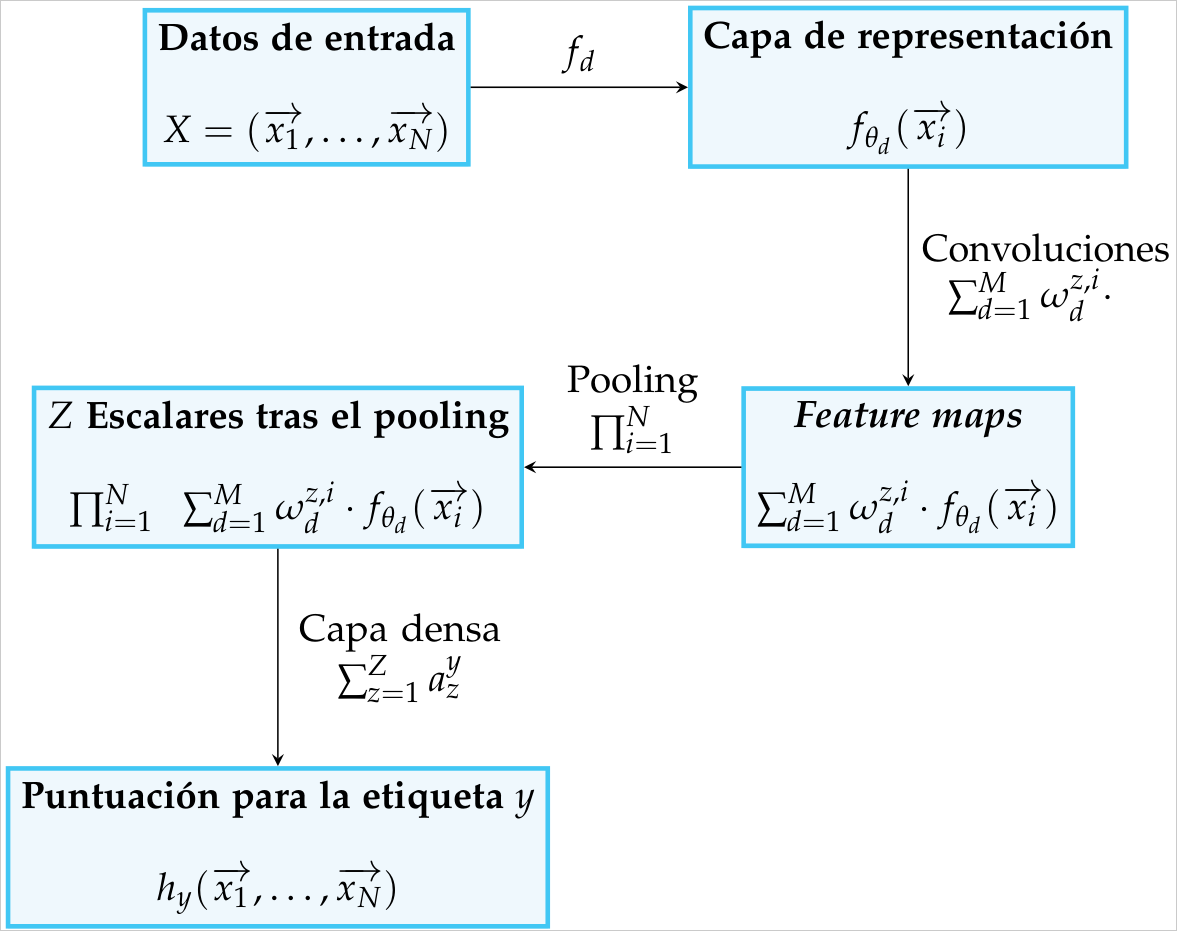
\includegraphics[width=0.7\textwidth]{matematicas/relacion_cnn_tikz}
		\caption{Representación gráfica del modelo \textit{CP}.}
	\end{figure}

\end{frame}


\subsection{Modelización de las redes profundas}
\begin{frame}{Descomposición HT}

	\begin{equation} \label{eq:descomposicion_ht}
		\begin{split}
			\phi^{1, j, \gamma} &:= \sum_{\alpha = 1}^{r_0} a_{\alpha}^{1, j, \gamma} \cdot \nv{\varphi^{2j-1, \alpha}} \otimes \nv{\varphi^{2j, \alpha}} \\
			\ldots \\
			\phi^{l, j, \gamma} &:= \sum_{\alpha = 1}^{r_{l-1}} a_{\alpha}^{l, j, \gamma} \cdot \phi^{l-1, 2j-1, \alpha} \otimes \phi^{l-1, 2j, \alpha} \\
			\ldots \\
			\mathcal{A}^y &:= \sum_{\alpha = 1}^{r_{L-1}} a_{\alpha}^{L, y} \cdot \phi^{L-1, 1, \alpha} \otimes \phi^{L-1, 2, \alpha}
		\end{split}
	\end{equation}

	\begin{itemize}
		\item $l$: nivel en la descomposición.
		\item $j$: posición dentro del nivel $l$.
		\item $\gamma$: tensor de la capa $l$ y posición $j$.
		\item $r_l$: cuántos tensores hay en cada posición $j$ de la capa $l$.
	\end{itemize}

\end{frame}

\begin{frame}{Primer ejemplo}

	\begin{figure}
		\centering
		
\includegraphics[width=0.7\textwidth]{matematicas/descomp_ht_rank_1}
		\caption{Ejemplo gráfico tomando $r = 1$, $L = 2$.}
		\label{img:diagrama_ht_simple}
	\end{figure}

\end{frame}

\begin{frame}{Segundo ejemplo}

	\begin{figure}
		
\includegraphics[width=0.7\linewidth]{matematicas/descomp_ht_rank_2_paso_1}
		\caption{Ejemplo gráfico tomando $r = 2$, $L = 2$ capas, primer paso.}
	\end{figure}

\end{frame}

\begin{frame}{Segundo ejemplo}

	\begin{figure}
		
\includegraphics[width=0.7\linewidth]{matematicas/descomp_ht_rank_2_paso_2}
		\caption{Ejemplo gráfico tomando $r = 2$, $L = 2$ capas, segundo paso.}
	\end{figure}

\end{frame}

\begin{frame}{Relación con arquitecturas de aprendizaje automático}

	\begin{figure}
		\centering
		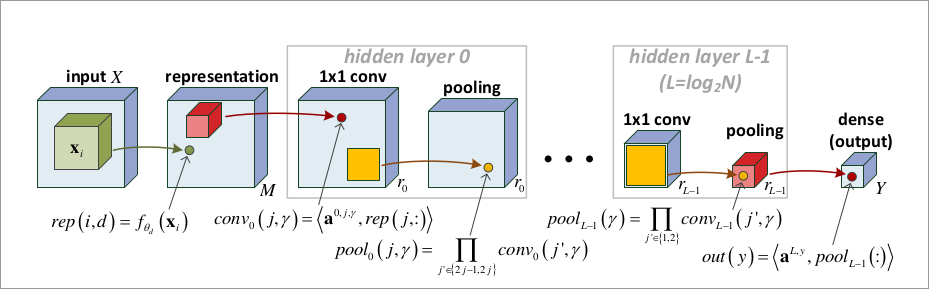
\includegraphics[width=0.9\textwidth]{matematicas/diagrama_paper_modelo_ht}
		\caption{Funcionamiento de nuestro modelo. Imagen extraída de \cite{matematicas:principal}.}
	\end{figure}


\end{frame}

\subsection{Resultados principales}

\begin{frame}{Primer resultado central}

	\begin{block}{Rango \textit{CP} exponencial de un modelo \textit{HT}}
		Sea $\mathcal{A}^y \in \espaciotensores{N}{M}$ dado por las ecuaciones \eqref{eq:descomposicion_ht}. Definamos $r := \min \conjunto{r_0, M}$ y consideremos el espacio de todas las posibles configuraciones de parámetros de nuestro modelo \textit{HT} $\conjunto{ \nv{a^{l, j, \gamma}}}_{l, j, \gamma}$. En este espacio, el tensor generado $\mathcal{A}^y$ tendrá rango \textit{CP} de al menos $r^{N/2}$ casi por doquier. Es decir, el conjunto de parámetros del modelo \textit{HT} con los que el modelo tiene rango \textit{CP} menor que $r^{N/2}$ tiene medida nula. El resultado se mantiene si forzamos los coeficientes compartidos en la ecuación \eqref{eq:descomposicion_ht}. Es decir, haciendo $\nv{a^{l, \gamma}} \equiv \nv{a^{l, j, \gamma}}$ y considerando el espacio de configuraciones $\{ \nv{a^{l, \gamma}}  \}_{l, \gamma}$.

	\end{block}


\end{frame}

\begin{frame}{Segundo resultado central}

	\begin{block}{Incapacidad del modelo \textit{CP} para aproximar eficientemente el modelo \textit{HT}}
		Dado un conjunto de funciones de representación linealmente independientes, $\conjunto{f_{\theta_d}: \; d \in \deltaset{M}}$, aleatorizar los pesos de un modelo \textit{HT} \eqref{eq:descomposicion_ht} a partir de una distribución de probabilidad continua induce funciones de puntuación $h_y$ que con probabilidad uno no pueden ser aproximadas arbitrariamente bien (en el sentido $L^2$) por un modelo \textit{CP} con menos de $r := \min \{r_0, M \}^{N/2}$ canales. Este resultado se mantiene forzando los coeficientes compartidos en el modelo \textit{HT} mientras que dejamos el modelo \textit{CP} sin restricciones.
	\end{block}

\end{frame}

\begin{frame}
	\begin{itemize}
		\item El primer resultado nos dice que casi todos los tensores $\mathcal{A}^y$ que podemos generar con un modelo \textit{HT} tienen rango \textit{CP} de al menos $r^{N/2}$, lo que implica que el modelo \textit{CP} necesita un número exponencial de parámetros.
		\item El segundo resultado añade a este hecho que ni siquiera pueden aproximarse eficientemente (menos de un número exponencial de coeficientes) por una descomposición \textit{CP}.
		\item Damos información precisa sobre cómo de frecuente ocurre este hecho (casi por doquier). Otros trabajos \cite{matematicas:descomposicion_ht} únicamente dan ejemplos concretos en los que esto ocurre.
	\end{itemize}
\end{frame}

\subsection{Conclusiones}
\begin{frame}{Conclusiones}
	Se han cumplido los objetivos iniciales.
\end{frame}

\section{Reconocimiento facial invariante a la edad}

\subsection{Objetivos}
\begin{frame}{Objetivos}

	\begin{itemize}
		\item Resolver una tarea de \textbf{reconocimiento facial invariante a cambios en la edad}, por sus siglas en inglés, \textit{AIFR}.
	\end{itemize}

	\begin{itemize}
		\item Estudiar dos \textbf{variantes \textit{online}} en la función de pérdida \textit{Triplet Loss}.
	\end{itemize}

\end{frame}

\subsection{Tarea a resolver}

\begin{frame}{\textit{AIFR}}

	\begin{figure}
		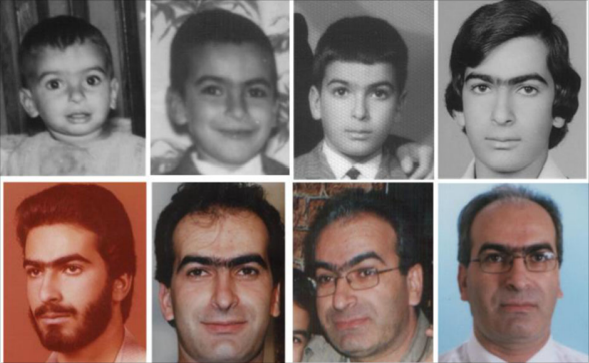
\includegraphics[width=0.8\textwidth]{informatica/ejemplo_dificultad_aifr}
		\caption{Ejemplo de datos con los que trabajamos en una tarea de \textit{AIFR}. Imagen extraída de \doblecita{informatica:aifr_survey}.}
		\label{img:ejemplo_dificultad_aifr}
	\end{figure}

\end{frame}

\begin{frame}{Problemas asociados a la tarea}

	\begin{figure}
		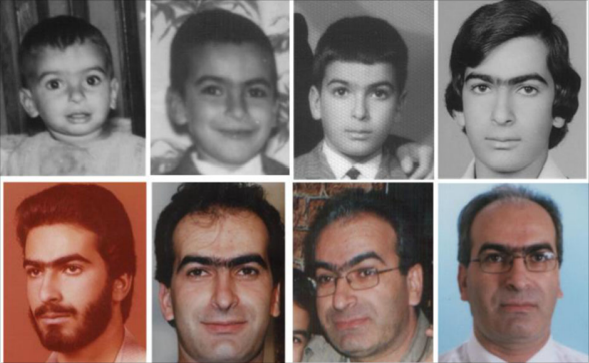
\includegraphics[height=0.4\textheight]{informatica/ejemplo_dificultad_aifr}
	\end{figure}

	\begin{itemize}
		\item Pueden ser más similares dos personas distintas de la misma edad que la misma persona en dos edades muy distantes.
		\item El envejecimiento modifica las características faciales.
		\item Trabajar con identidades nunca vistas.
		\item Escasez de conjuntos de datos para estudiar la tarea de \textit{AIFR}, que además presentan diversas dificultades.
	\end{itemize}

\end{frame}

\subsection{Enfoque}

\begin{frame}{Embedding semántico}
	\begin{columns}
		\column{0.6\linewidth}
		\centering
		\begin{figure}
			\includegraphics[width=0.8\textwidth]{informatica/embedding_paper_principal}
		\end{figure}
		\column{0.5\linewidth}
		\begin{itemize}
			\item Queremos que nuestra red aprenda un \textbf{\textit{embedding} semántico}.
			\item Elementos de la misma identidad deberán estar cerca entre sí, mientras que elementos de distintas identidades deberán estar distantes.
		\end{itemize}
	\end{columns}
	Imagen extraída de \doblecita{informatica:principal}.
\end{frame}

\begin{frame}{Embedding Semántico}
	\begin{figure}
		\includegraphics[height=1.0\textheight]{informatica/embedding_paper_principal}
	\end{figure}
\end{frame}

\begin{frame}{Redes siamesas}

	\begin{figure}
		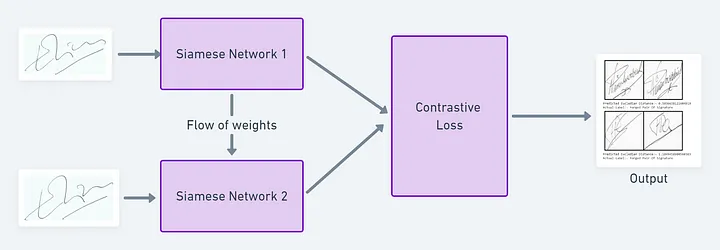
\includegraphics[width=0.9\textwidth]{informatica/siamesa_firma}
		\caption{Imagen extraída de \doblecita{informatica:siamesa_web_imagen}.}
		\label{img:siamesa_firma}
	\end{figure}

	\begin{itemize}
		\item Herramienta para aprender el \textit{embedding}.
		\item Se utiliza o \textit{contrastive loss} (pares) o \textit{triplet loss} (triples).
	\end{itemize}

\end{frame}

\begin{frame}{Triplet Loss}
	\begin{figure}
		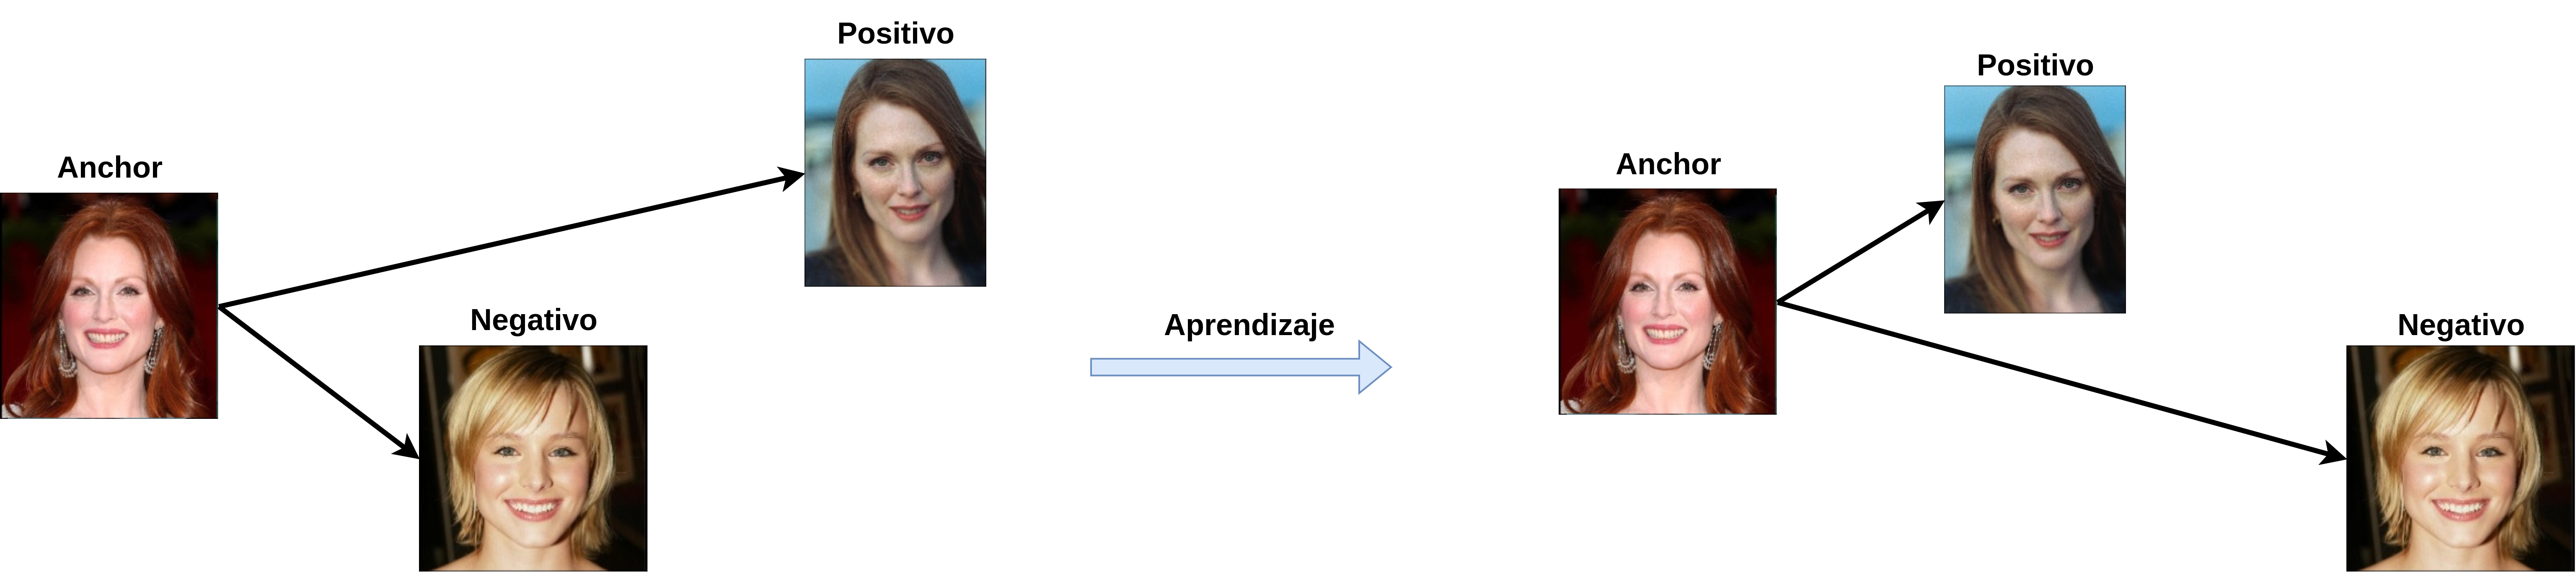
\includegraphics[width=1.0\textwidth]{informatica/triplet_loss_learning}
		\caption{Imágenes extraídas de \doblecita{informatica:cacd_dataset}.}
	\end{figure}

	A partir de:
	\begin{equation}
		D_{A, P} \leq D_{A, N},
	\end{equation}

	llegamos a:

	\begin{equation} \label{ieq:triplet_loss_single_entry}
		\mathcal{L}_{tri}(\theta; A, P, N) := max \{D_{A, P} - D_{A, N} + \alpha, 0 \}
	\end{equation}
\end{frame}

\begin{frame}{Variantes \textit{online} sobre \textit{Triplet Loss}}

	\begin{itemize}
		\item Problema: necesitamos generar los triples de forma \textit{offline}.
		\item Solución: generar los \textit{batches} de forma \textit{online}.
		      \begin{itemize}
			      \item Usando \textit{P-K} sampling.
			      \item Aplicando las variantes \textit{Batch All} y \textit{Batch Hard} sobre estos nuevos \textit{batches}
		      \end{itemize}
	\end{itemize}

	\begin{figure}
		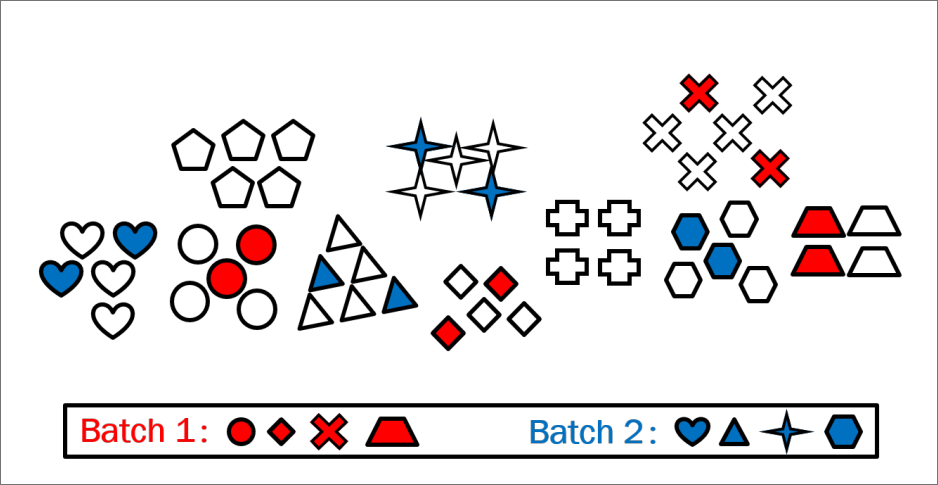
\includegraphics[width=0.6\textwidth]{informatica/ejemplo_grafico_pk_sampling}
		\caption{Imagen extraída de \doblecita{informatica:paper_image_pk_sampling}.}
	\end{figure}

\end{frame}

\begin{frame}{Variantes \textit{online}}

	Sobre el anterior \textit{P-K} sampling:

	\begin{itemize}
		\item \textbf{\textit{Batch All}}: probar todas las combinaciones ancla - positivo - negativo.
		\item \textbf{\textit{Batch Hard}}: por cada ancla, computar la pérdida con el positivo más lejano y el negativo más cercano (combinación más complicada).
	\end{itemize}

\end{frame}

\subsection{Experimentación preliminar}
\begin{frame}{Métricas más relevantes}
	\begin{itemize}
		\item \textit{Rank@k}: dada una imagen de entrada, la red devuelve las $k$ imágenes que detecta como más cercanas. Contamos como acierto si al menos una imagen corresponde a la identidad apropiada.
		\item \textit{Silhouette}: mide la calidad de los \textit{clusters} o agrupaciones obtenidas. Va desde -1 (peor valor) hasta 1 (valor perfecto).
	\end{itemize}
\end{frame}

\begin{frame}{\textit{CACD}}

	\begin{figure}
		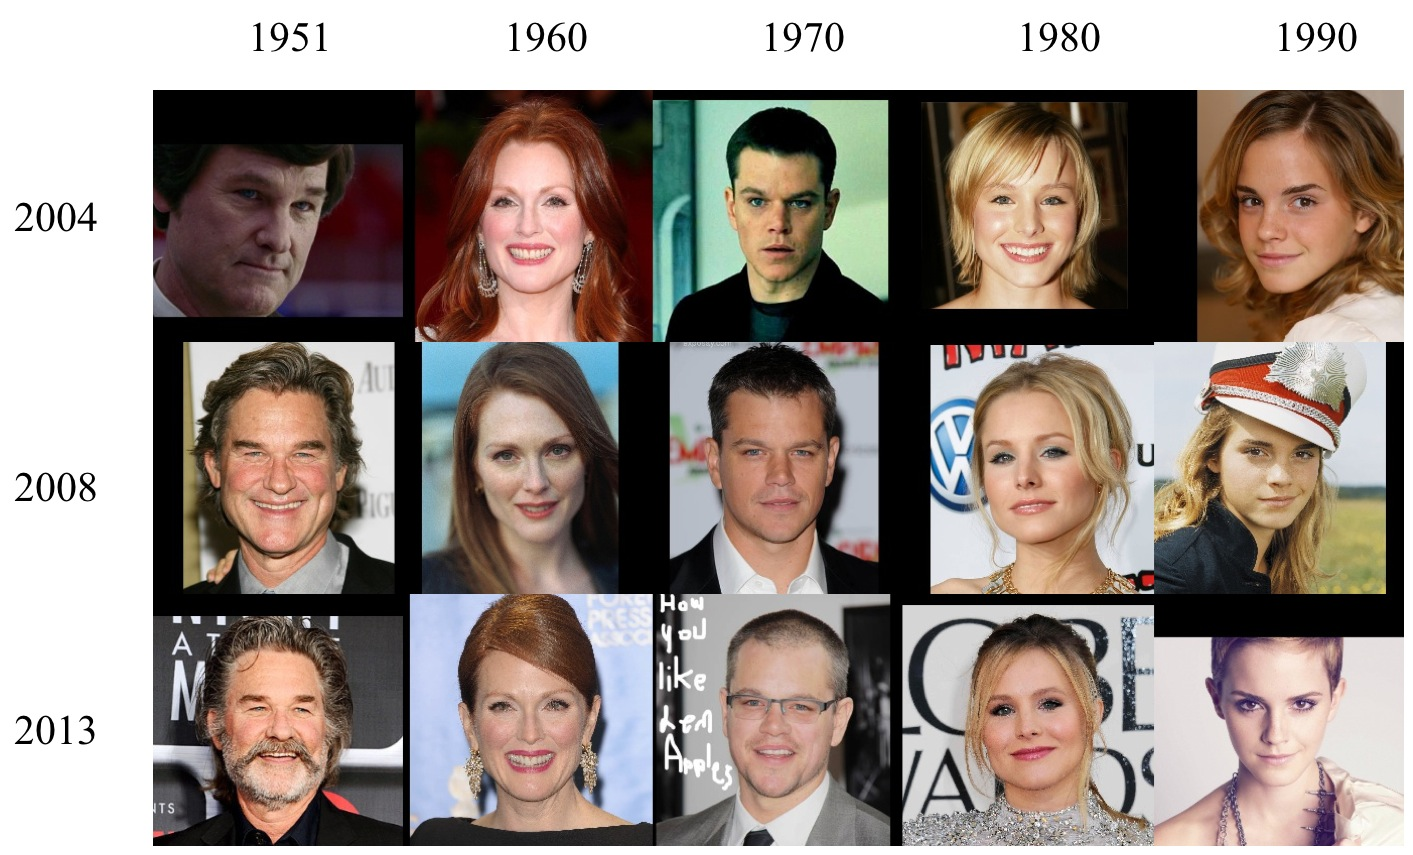
\includegraphics[width=0.9\textwidth]{informatica/cacd_example}
		\caption{Imagen extraída de \doblecita{informatica:paper_cacd}}
		\label{img:cacd_imagenes_ejemplo}
	\end{figure}

\end{frame}

\begin{frame}{Resultados preliminares sobre \textit{CACD}}
	\begin{figure}
		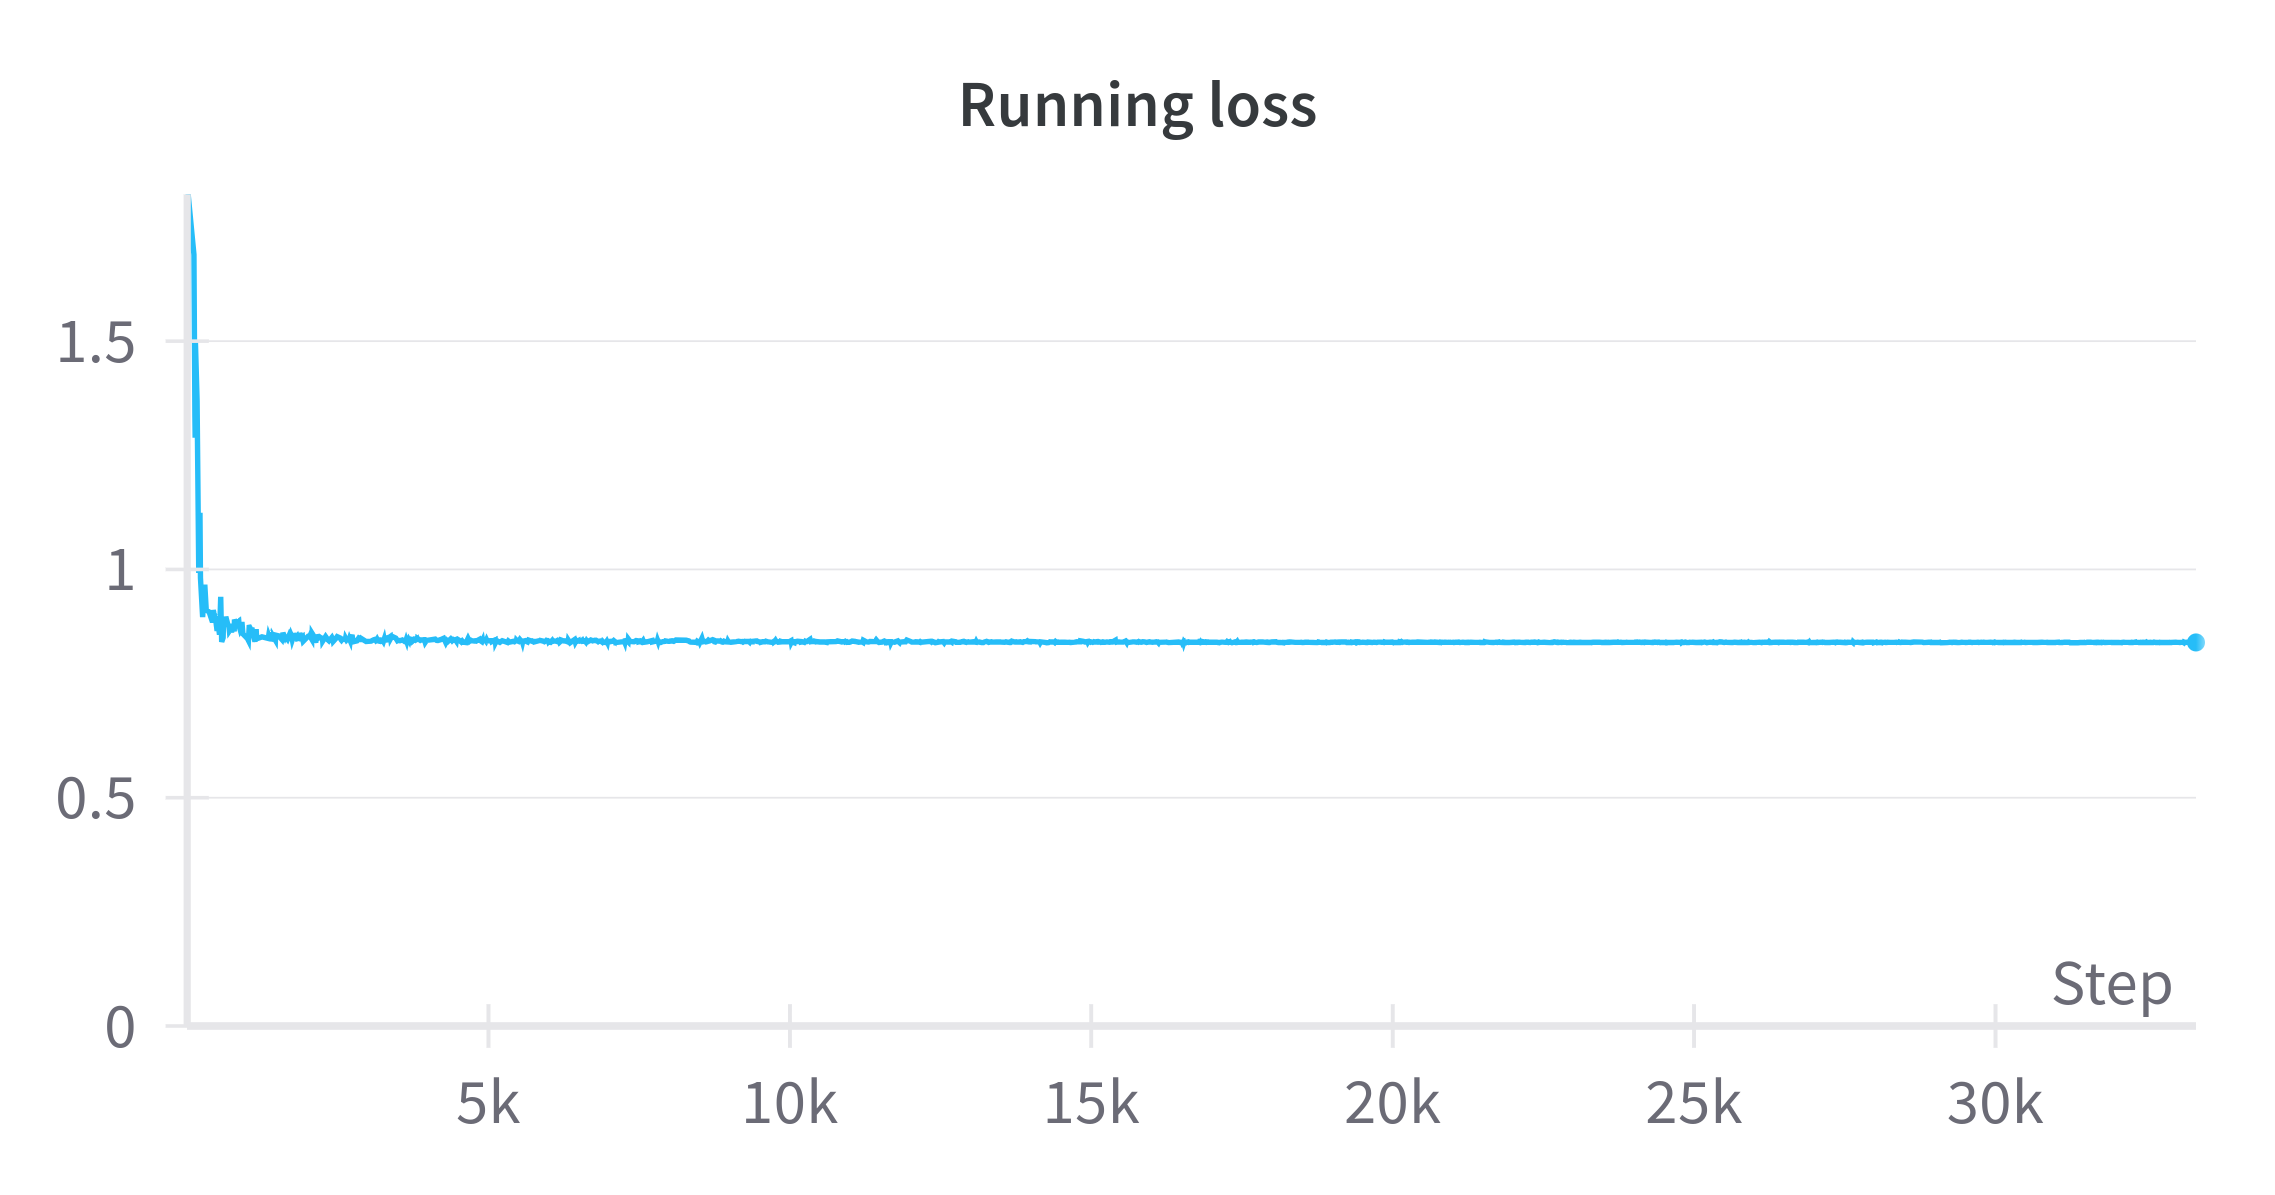
\includegraphics[width=1.0\textwidth]{informatica/wandb/entrenamiento_principal/running_loss}
	\end{figure}
\end{frame}

\begin{frame}{Resultados preliminares sobre \textit{CACD}}
	\begin{figure}
		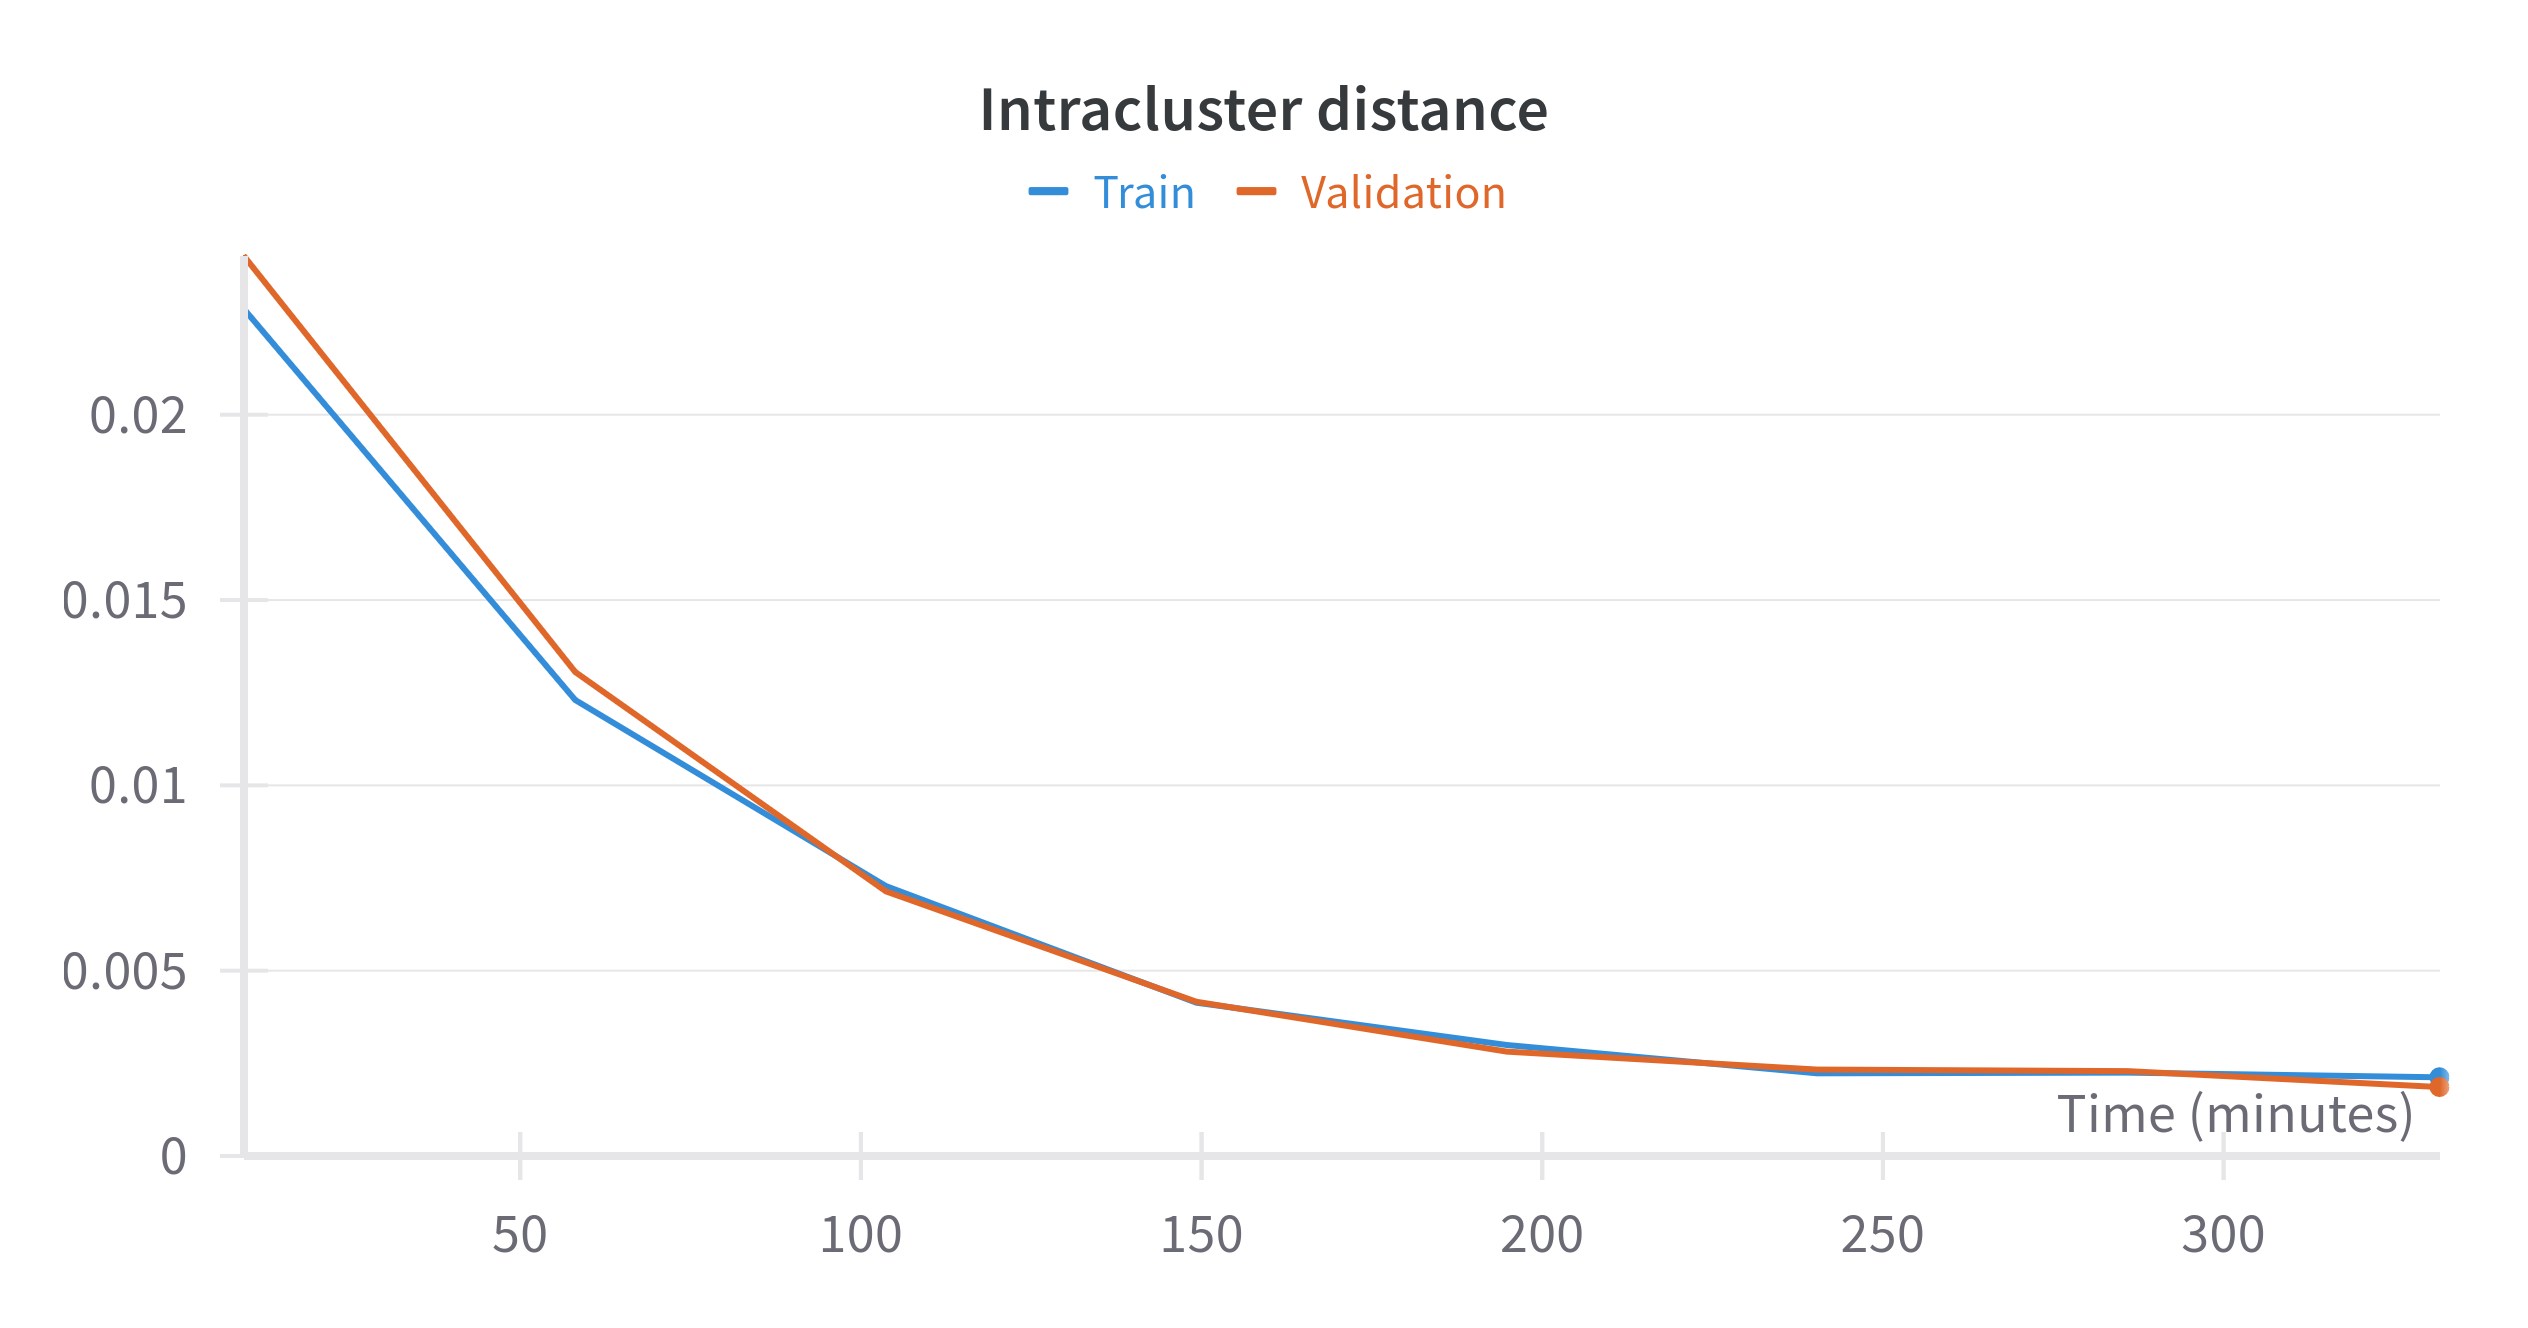
\includegraphics[width=1.0\textwidth]{informatica/wandb/entrenamiento_principal/intracluster_distance}
	\end{figure}
\end{frame}

\begin{frame}{Resultados preliminares sobre \textit{CACD}}
	\begin{figure}
		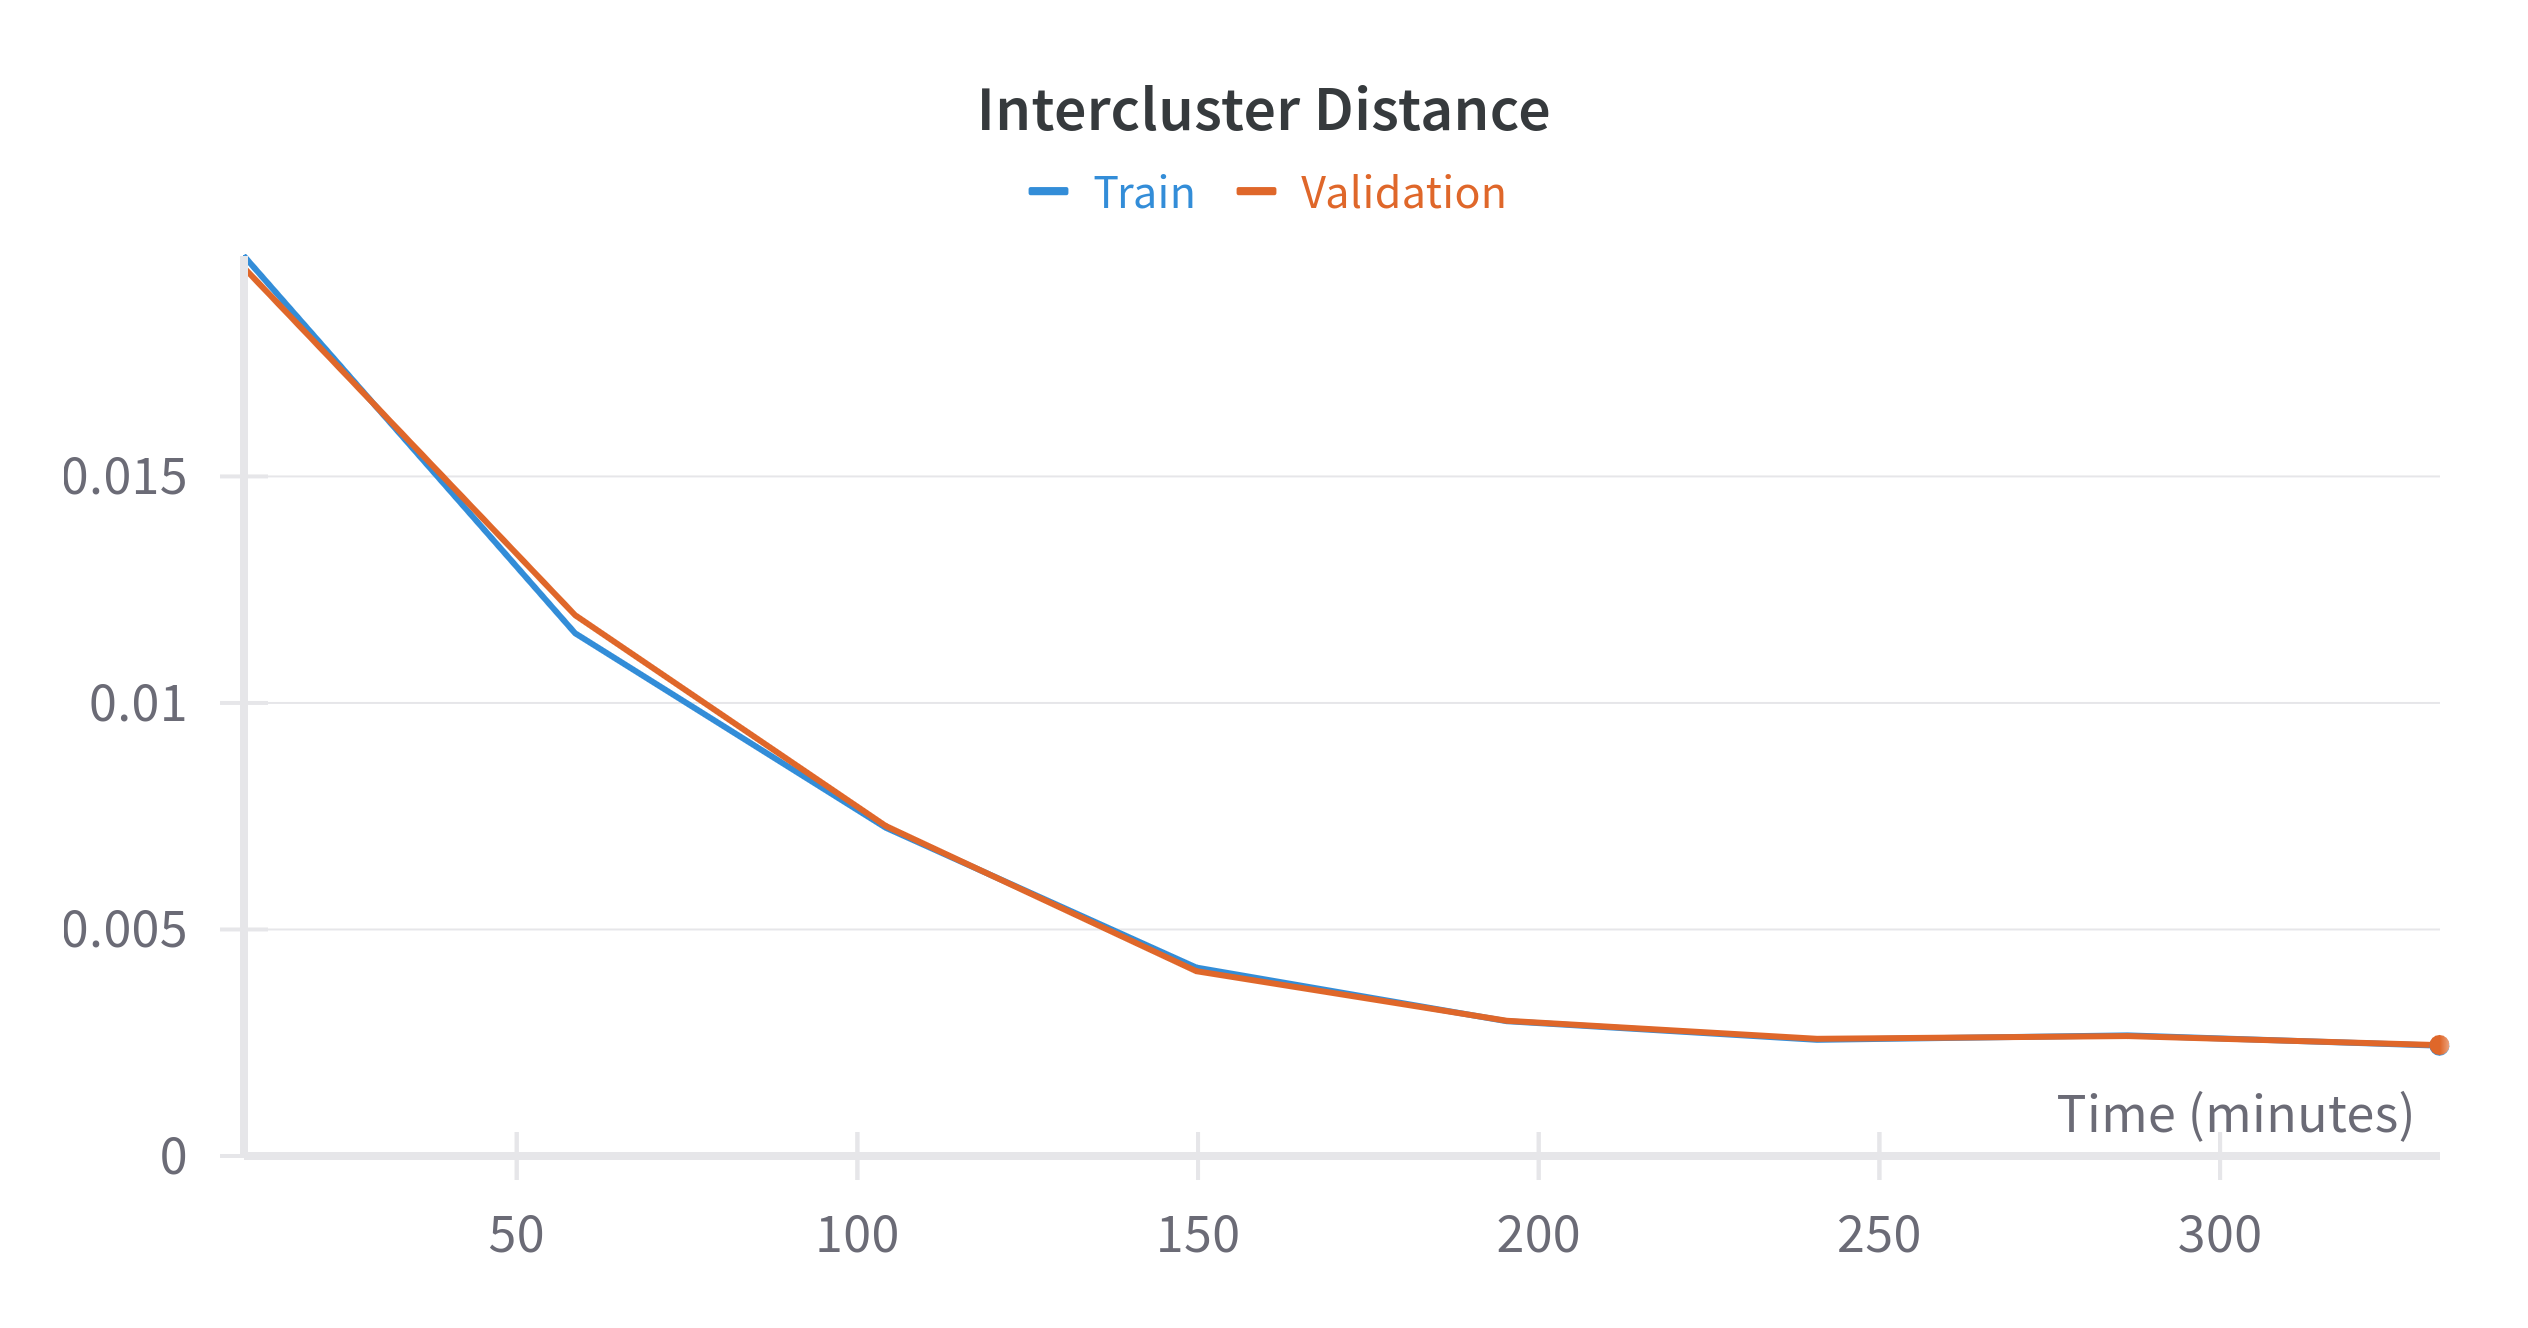
\includegraphics[width=1.0\textwidth]{informatica/wandb/entrenamiento_principal/intercluster_distance}
	\end{figure}

\end{frame}

\begin{frame}{Resultados preliminares sobre \textit{CACD}}
	\begin{table}
		\centering
		\begin{tabular}{|l|l|l|l|}
			\hline
			Conjunto      & \textit{Rank@1 Accuracy} & \textit{Rank@5 Accuracy} & \textit{Silhouette} \\
			\hline

			Entrenamiento & 0.07185                  & 0.15244                  & -0.41858            \\
			Test          & 0.01000                  & 0.00100                  & -0.32984            \\
			\hline
		\end{tabular}
		\caption{Valores de distintas métricas obtenidas sobre el conjunto \textit{CACD} de entrenamiento y sobre el conjunto \textit{FG-Net} de \textit{test}.}
		\label{table:resultados_sobre_fg_net}
	\end{table}

\end{frame}

\begin{frame}{Resultados preliminares sobre \textit{MNIST}}

	\begin{table}
		\centering
		\begin{tabular}{|l|l|l|l|}
			\hline
			Conjunto      & \textit{Rank@1 Accuracy} & \textit{Rank@5 Accuracy} & \textit{Silhouette} \\
			\hline

			Entrenamiento & 0.0937                   & 0.453                    & 0.000               \\
			Test          & 0.085                    & 0.414                    & 0.000               \\


			\hline
		\end{tabular}
		\caption{Métricas de evaluación obtenidas tras entrenar el modelo sobre \textit{MNIST}.}
		\label{table:resultados_mnist_mal}
	\end{table}

	En la experimentación realizada por \doblecita{informatica:adambielski_github} observamos los mismos problemas que estamos exponiendo.

\end{frame}

\subsection{Solución original}
\begin{frame}{Raíz del problema y nuestra propuesta de solución}
	\begin{itemize}
		\item La red aprende a transformar todas las entradas a un vector no nulo del \textit{embedding}.
		\item En esta situación tenemos que:
	\end{itemize}

	\begin{equation} \label{eq:justificacion_relu}
		\begin{split}
			\mathcal{L}(a, p, n) &= ReLU(d(a, p) - d(a, n) + \alpha) \\
			&= ReLU(d(\nv{v_0}, \nv{v_0}) - d(\nv{v_0}, \nv{v_0}) + \alpha) \\
			&= ReLU(0 - 0 + \alpha) = ReLU(\alpha) = \alpha.
		\end{split}
	\end{equation}

	\begin{itemize}
		\item Penalizar las distancias negativas pequeñas dividiendo por su media en el término ancla - positivo.
	\end{itemize}
	\begin{equation}
		\mathcal{L}(a, p, n) = \widehat{ReLU}((\widehat{d}(a, p) - \widehat{d}(a, n)) / mean(d(a, n)) + \alpha)
	\end{equation}

\end{frame}

\subsection{Validación experimental de nuestra solución}
\begin{frame}{Resultados en \textit{MNIST} con nuestra solución}

	\begin{figure}
		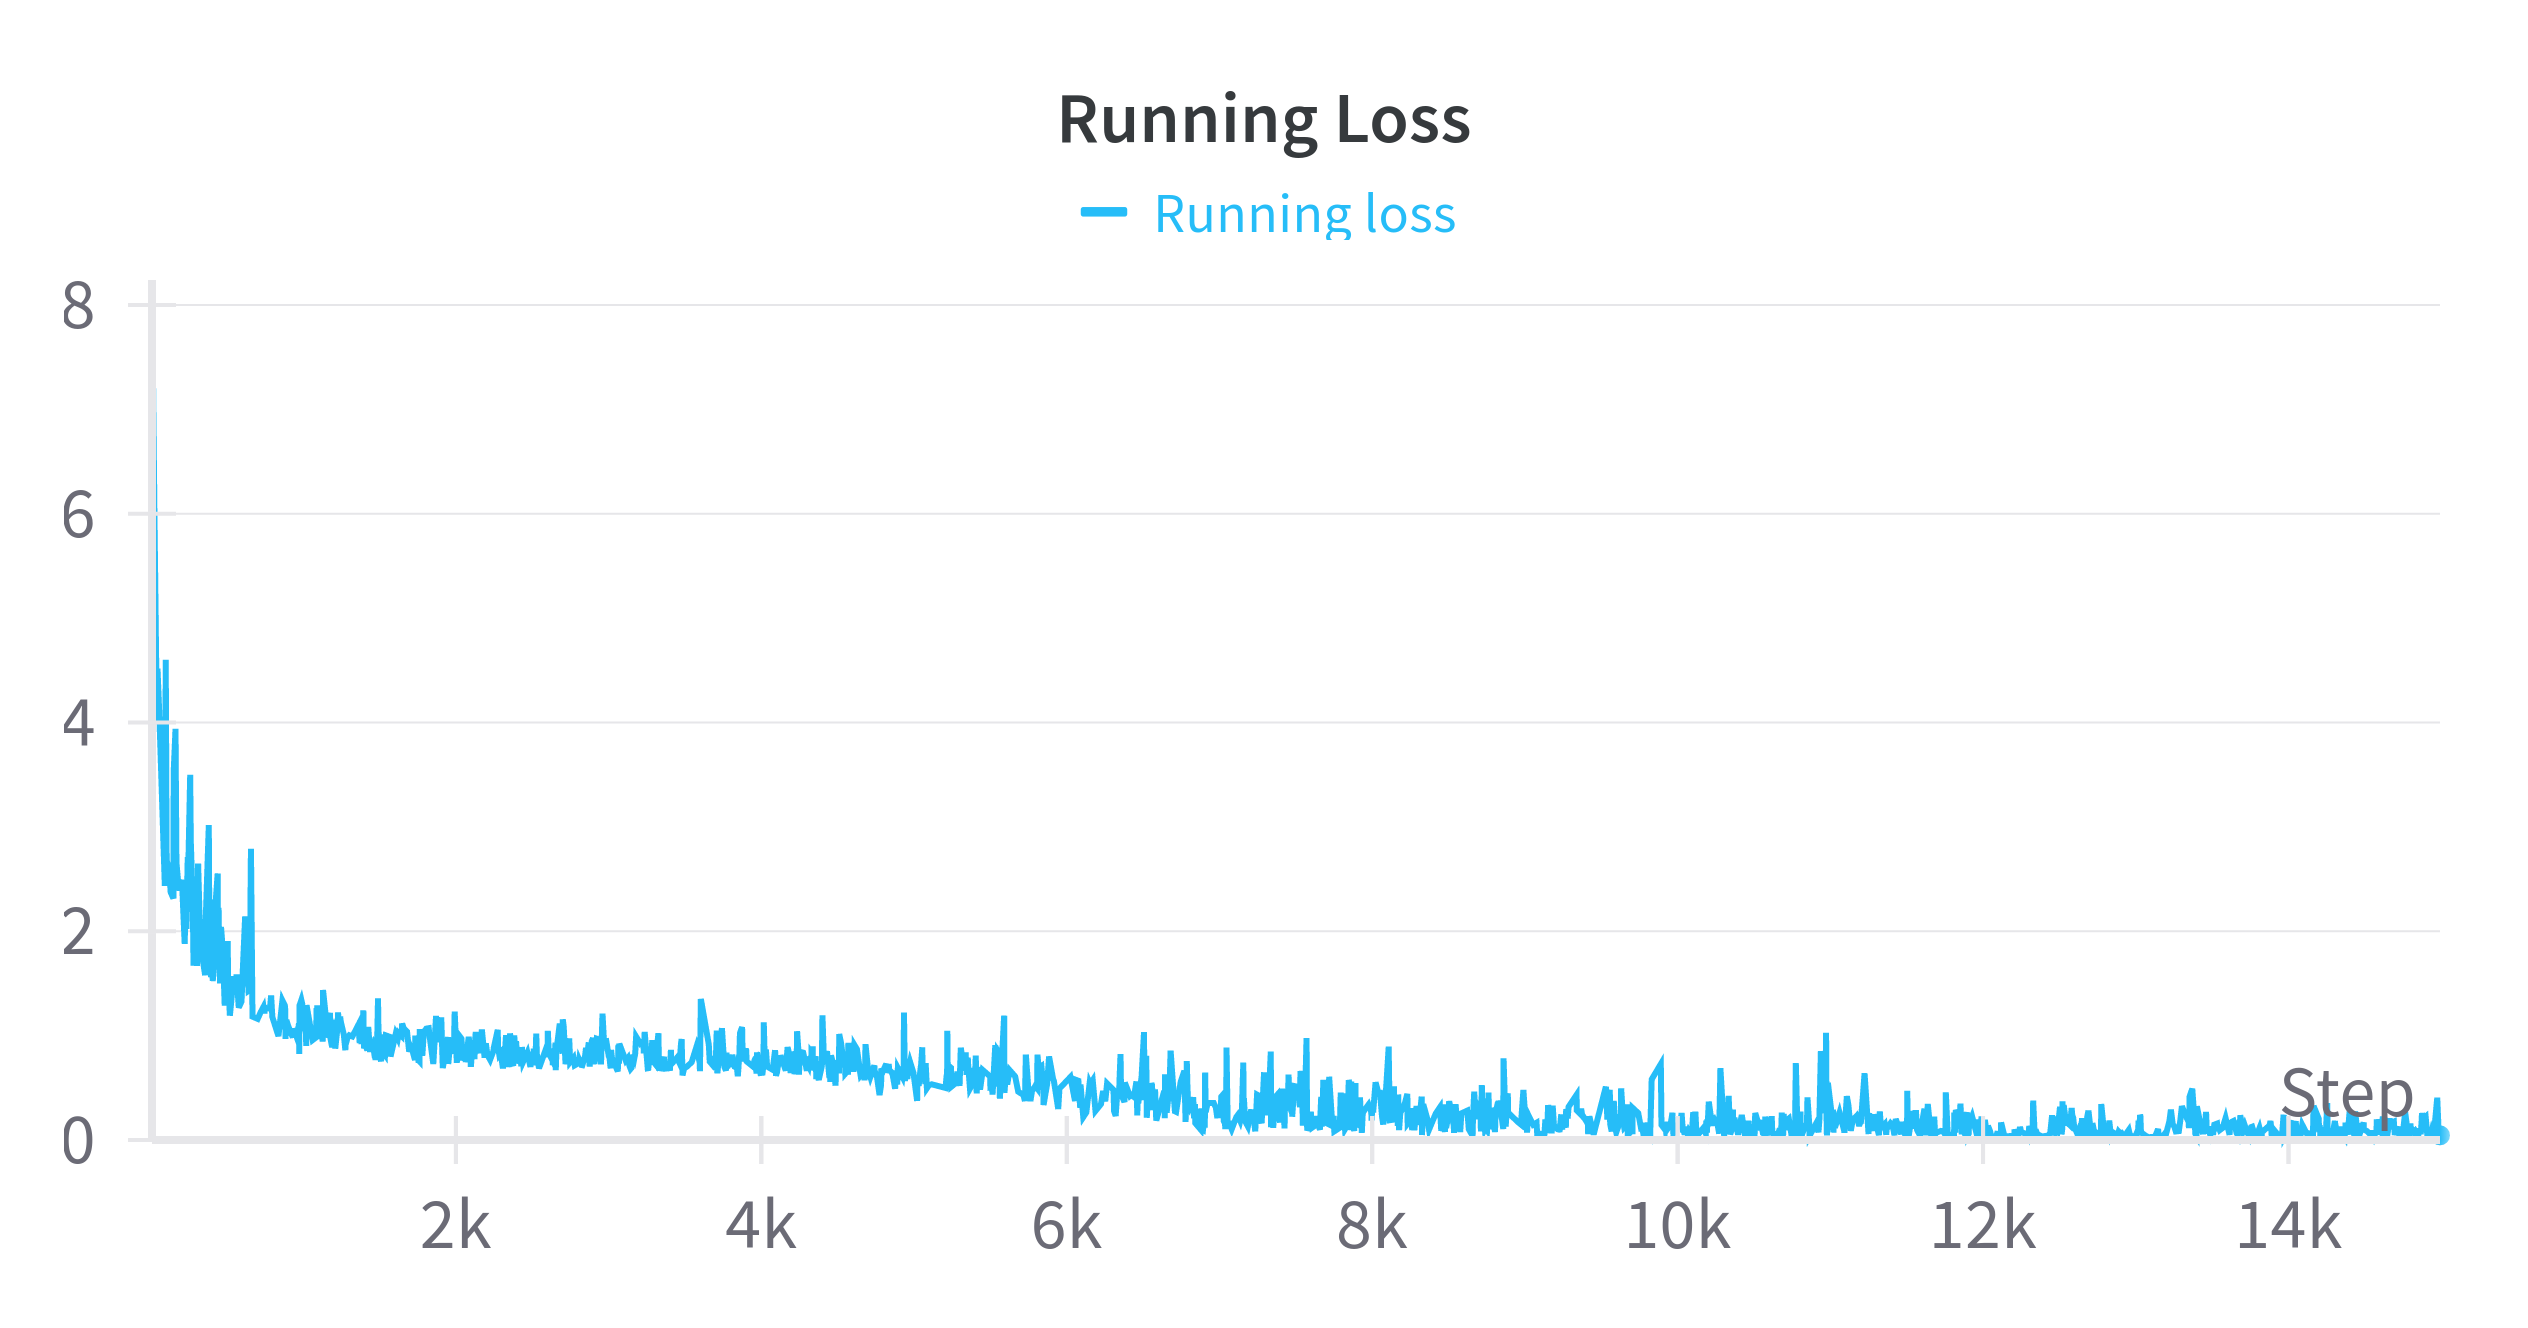
\includegraphics[width=0.8\linewidth]{informatica/wandb/mnist_corregido/batch_hard_running_loss.png}
	\end{figure}
\end{frame}

\begin{frame}{Resultados en \textit{MNIST} con nuestra solución}

	\begin{figure}
		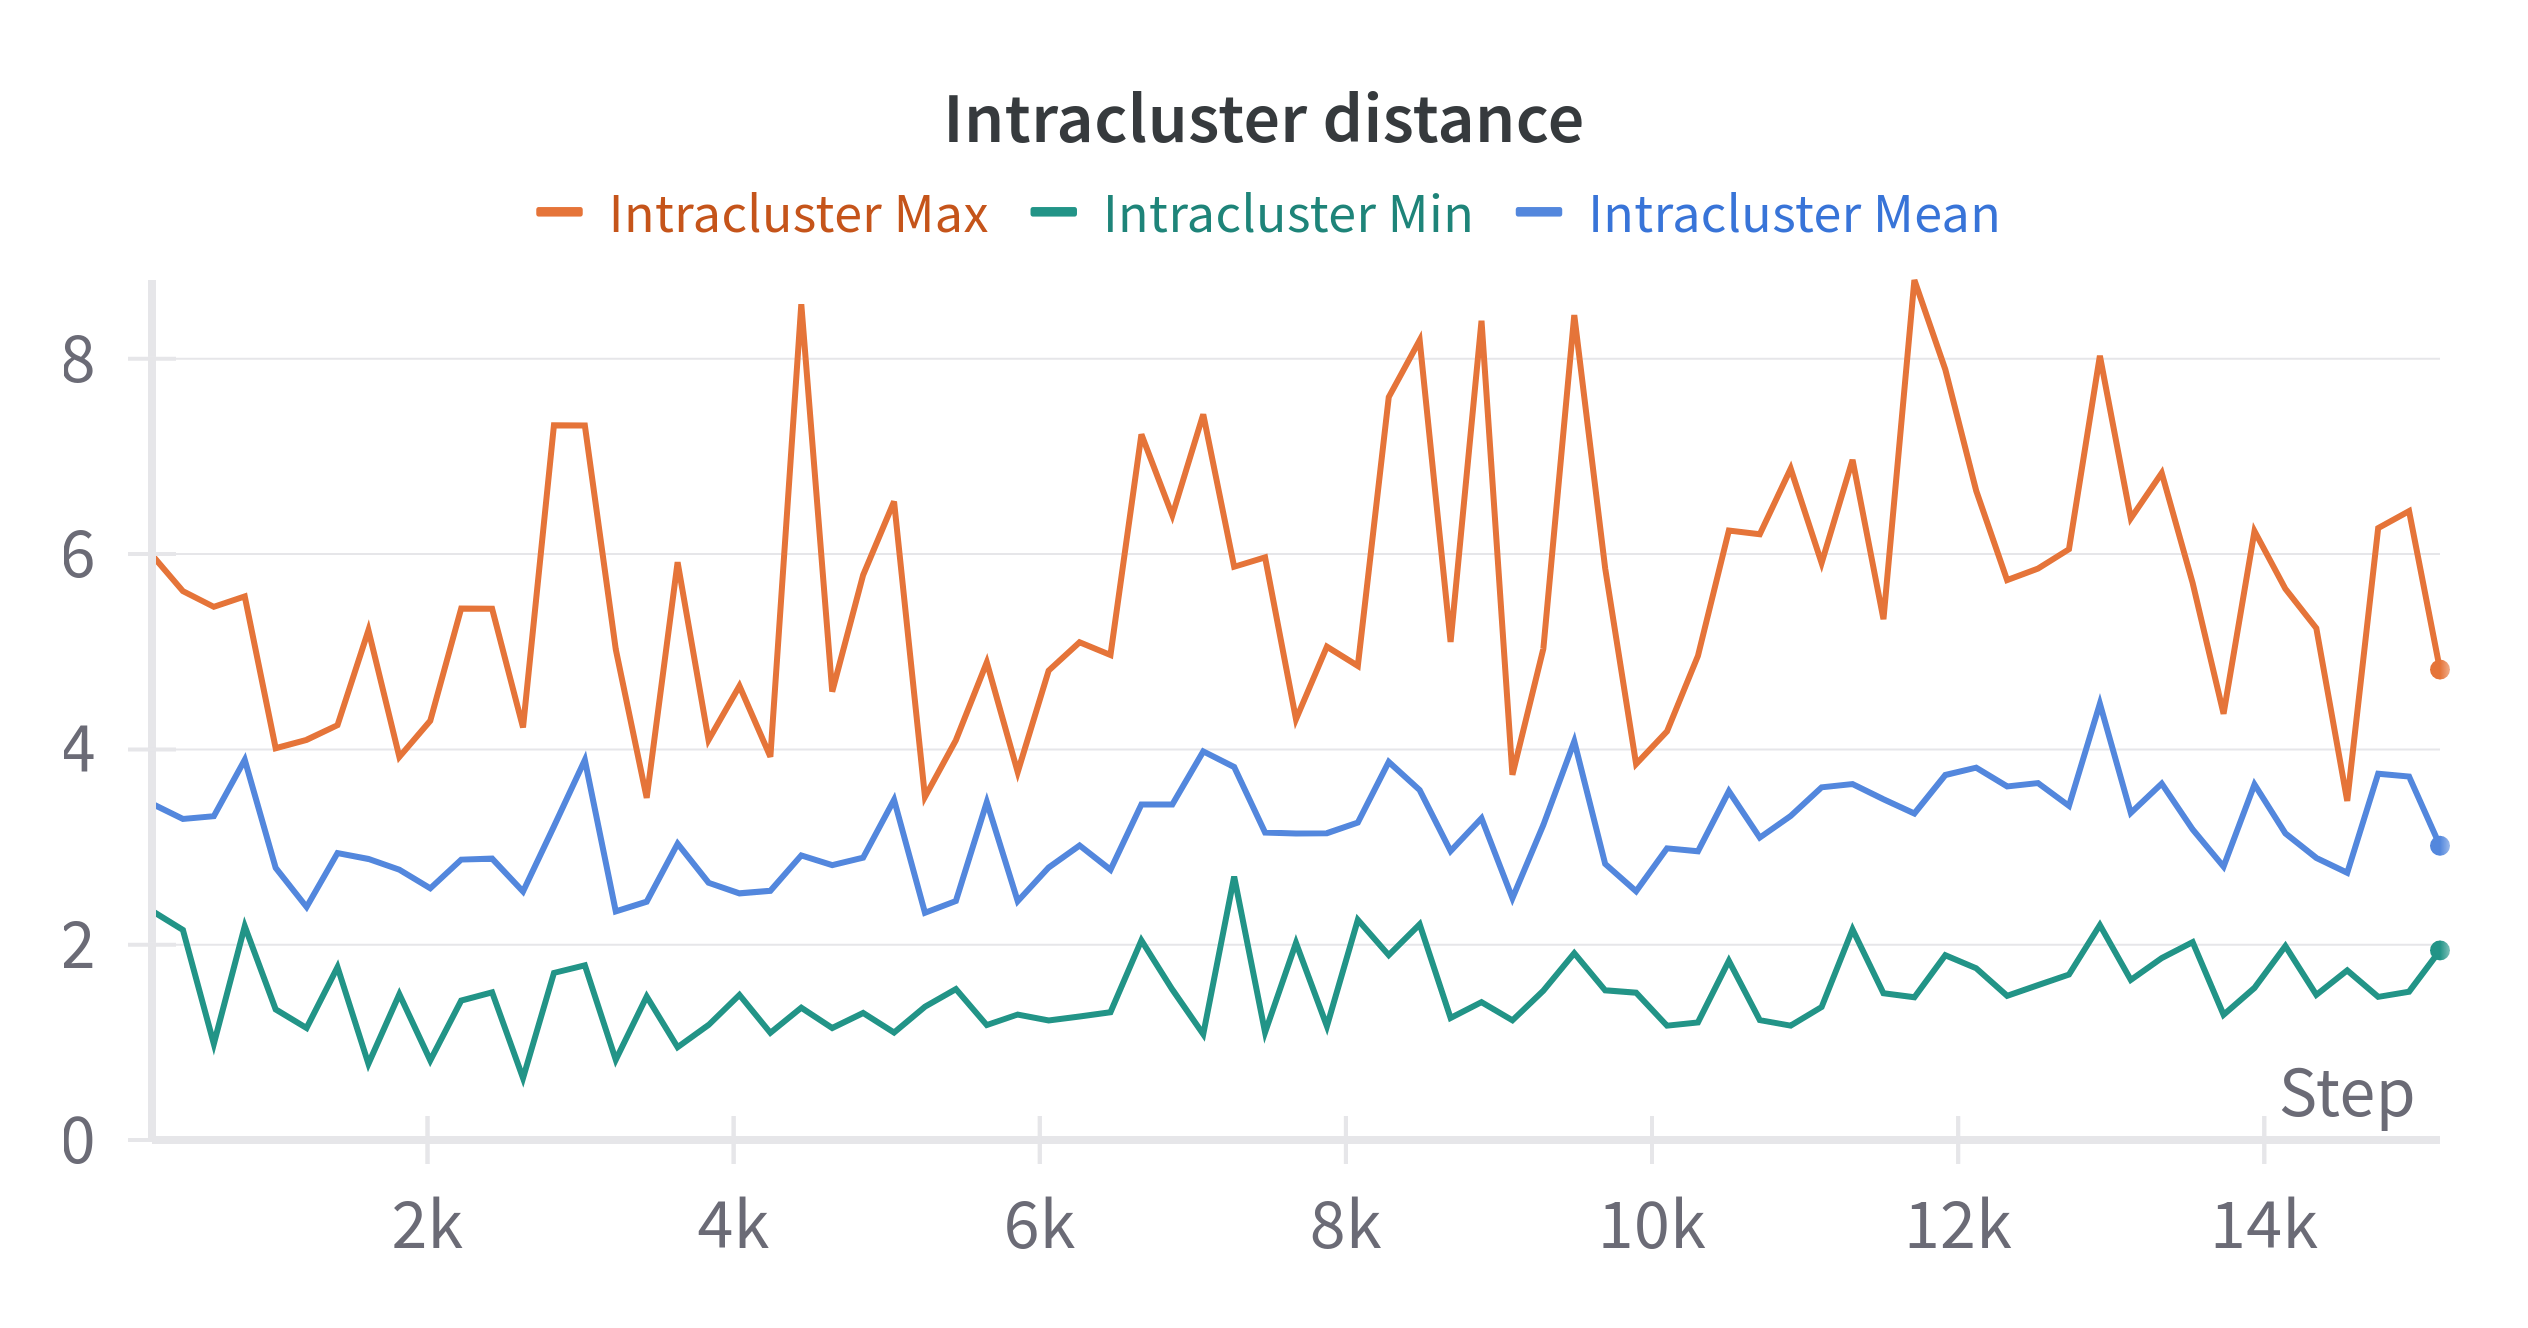
\includegraphics[width=0.8\linewidth]{informatica/wandb/mnist_corregido/batch_hard_intracluster.png}
	\end{figure}

\end{frame}

\begin{frame}{Resultados en \textit{MNIST} con nuestra solución}


	\begin{figure}
		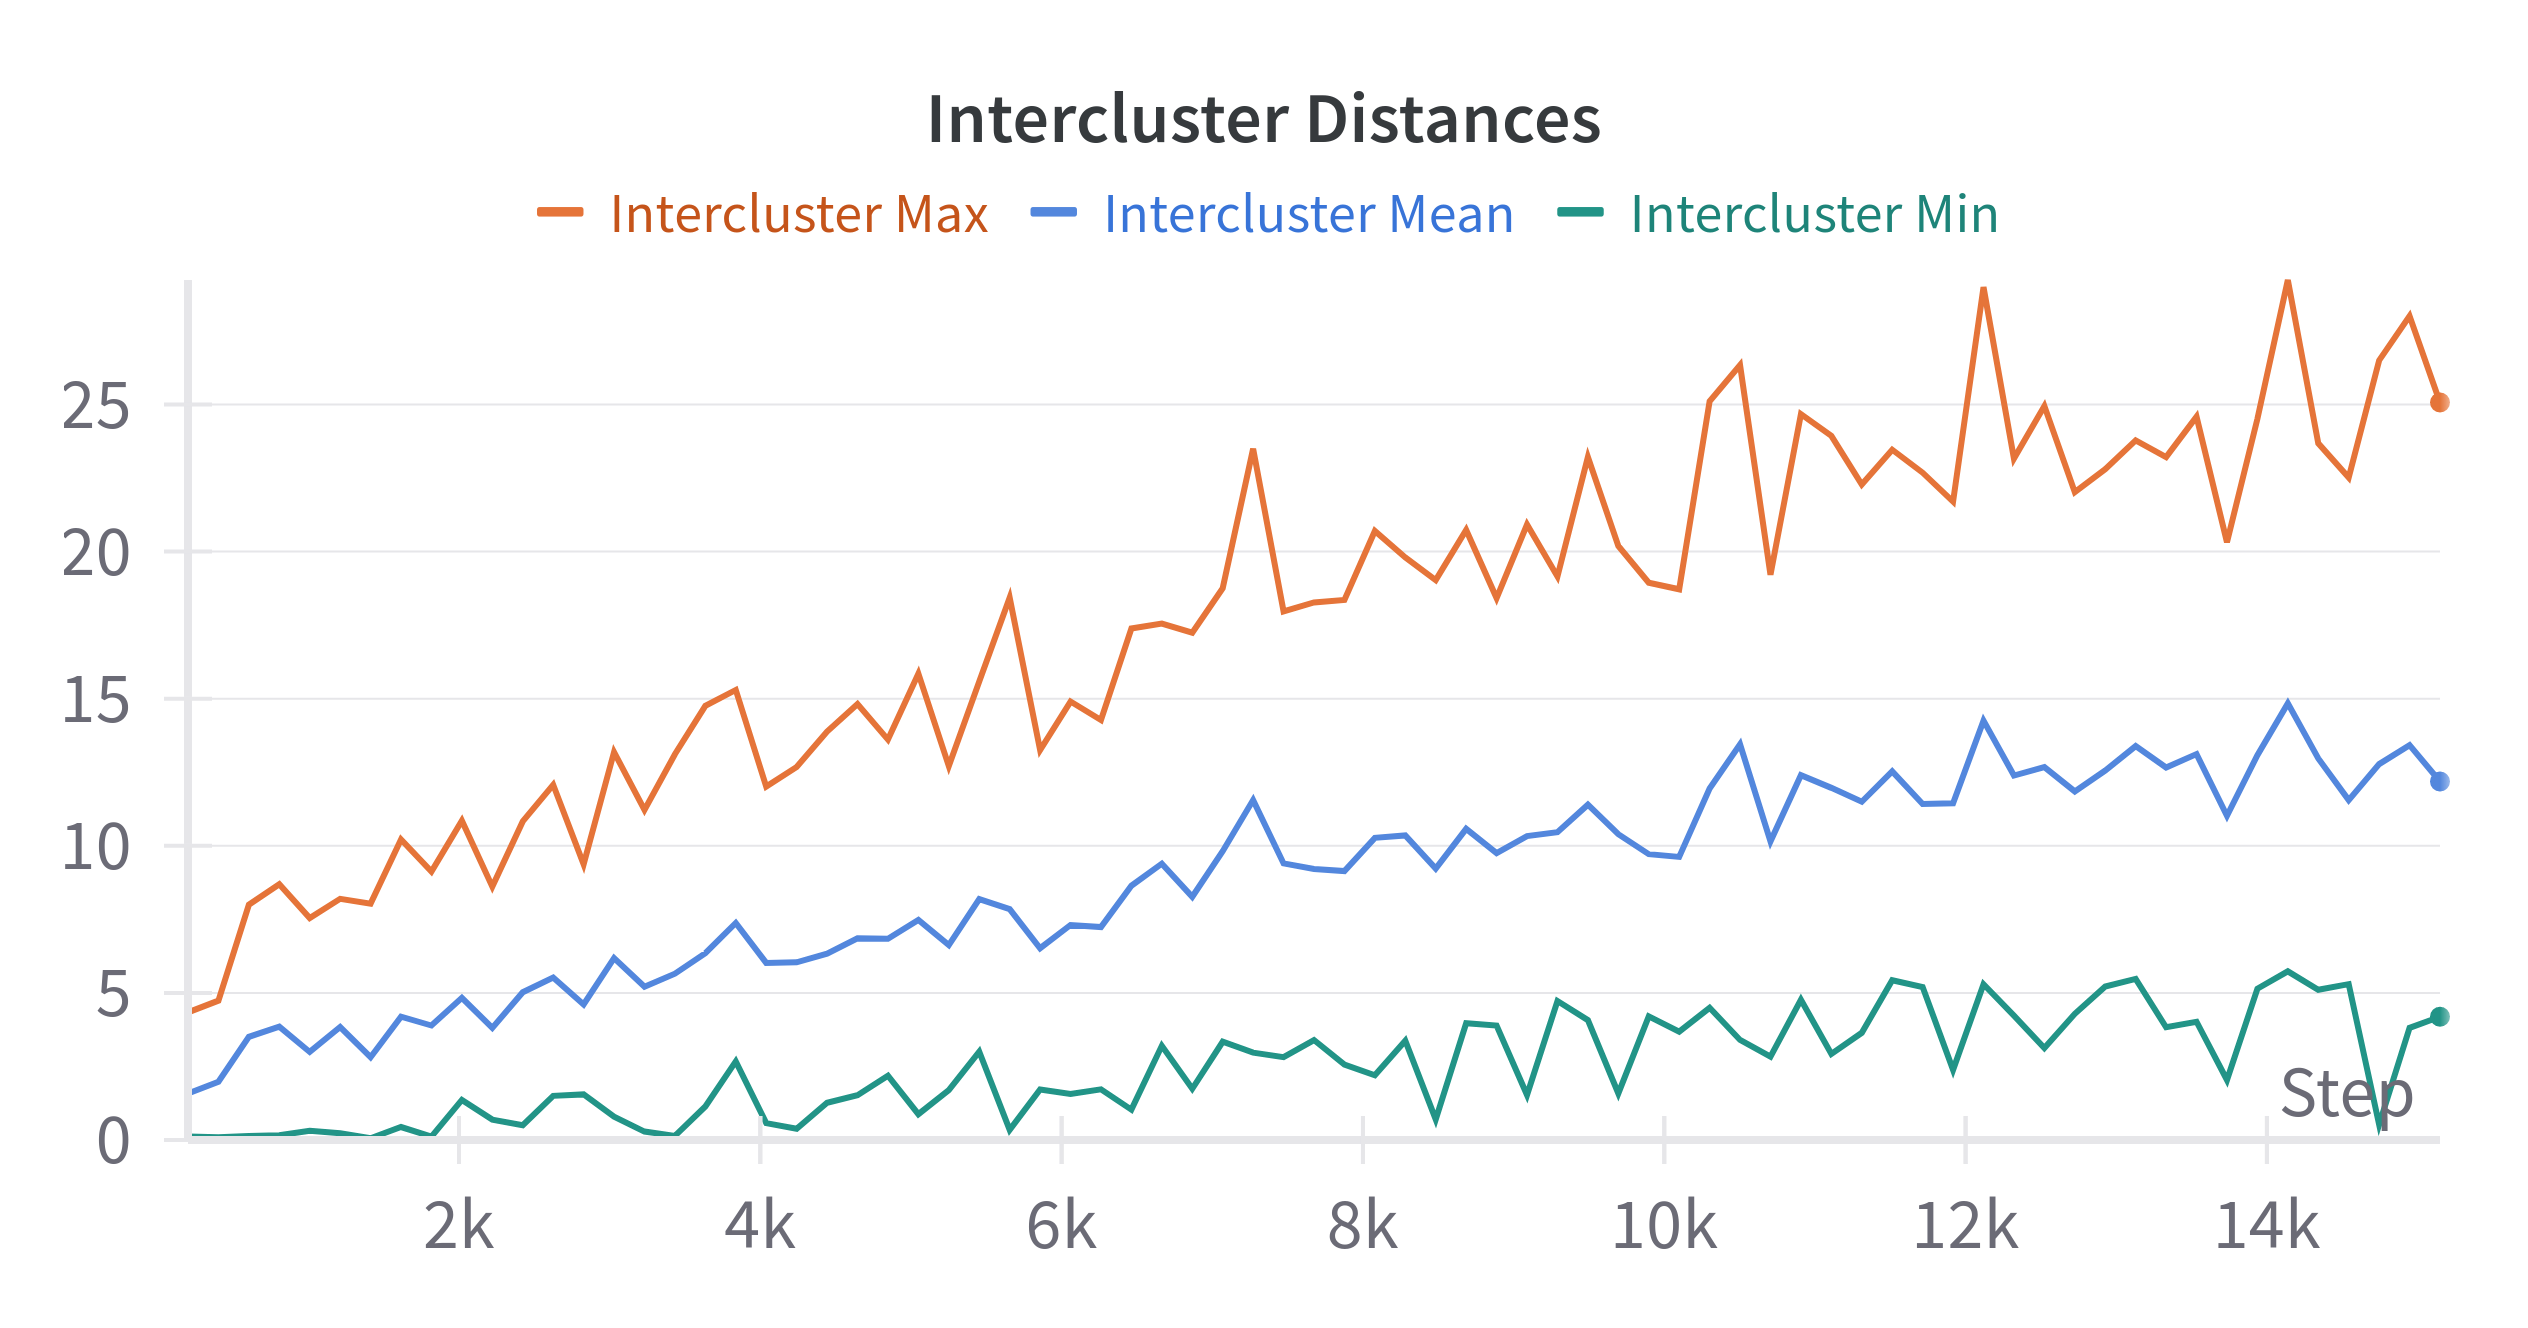
\includegraphics[width=0.8\linewidth]{informatica/wandb/mnist_corregido/batch_hard_interclusater.png}
	\end{figure}


\end{frame}

\begin{frame}{Mejora de los resultados en \textit{MNIST}}


	\begin{table}
		\centering
		\begin{tabular}{|l|l|l|l|l|}
			\hline
			Métrica                  & Conjunto      & Antes  & Después & Mejora   \\
			\hline
			\textit{Rank@1 Accuracy} & Entrenamiento & 0.0937 & 0.997   & 10.64    \\
			\textit{Rank@1 Accuracy} & Test          & 0.085  & 0.992   & 11.67    \\
			\textit{Rank@5 Accuracy} & Entrenamiento & 0.453  & 0.997   & 2.20     \\
			\textit{Rank@5 Accuracy} & Test          & 0.414  & 0.991   & 2.39     \\
			\textit{Silhouette}      & Entrenamiento & 0.000  & 0.953   & $\infty$ \\
			\textit{Silhouette}      & Test          & 0.000  & 0.922   & $\infty$ \\
			\hline
		\end{tabular}
		\label{table:comparaciones_mnist_resultados}
	\end{table}
\end{frame}

\begin{frame}{Mejora de los resultados en \textit{CACD}}

	\begin{table}
		\centering
		\begin{tabular}{|l|l|l|l|l|}
			\hline
			Métrica                  & Conjunto      & Antes   & Después & Mejora \\
			\hline
			\textit{Rank@1 Accuracy} & Entrenamiento & 0.0092  & 0.2676  & 29.09  \\
			\textit{Rank@1 Accuracy} & Test          & 0.0312  & 0.3732  & 11.96  \\
			\textit{Rank@5 Accuracy} & Entrenamiento & 0.0136  & 0.4639  & 34.11  \\
			\textit{Rank@5 Accuracy} & Test          & 0.0781  & 0.6152  & 7.88   \\
			\textit{Silhouette}      & Entrenamiento & -0.1366 & -0.1648 & -0.02  \\
			\textit{Silhouette}      & Test          & -0.1596 & -0.1832 & -0.023 \\
			\hline
		\end{tabular}
		\label{table:comparaciones_cacd_resultados}
	\end{table}


\end{frame}

\subsection{Conclusiones}
\begin{frame}{Conclusiones}

	\begin{itemize}
		\item Hemos identificado un problema de diseño en las variantes \textit{online} de \textit{Triplet Loss}.
		\item Hemos propuesto una solución original y validado experimentalmente su gran eficacia.
		\item Obtenemos buenos resultados en la tarea de \textit{AIFR}.
		\item Desarrollo en abierto de toda la base de código en nuestro repositorio de \textit{Github} \doblecita{informatica:repogithub}.
	\end{itemize}

\end{frame}

\section{Bibliografía}

\begin{frame}{Bibliografía Principal}

	\printbibliography[keyword={importante}]

\end{frame}


% Close with the titlepage again
\begin{frame}
	\titlepage
\end{frame}

\end{document}
